\chapter{Dataset}
\label{chap:data}
\section{Overview}

The dataset consists of chest X-ray (CXR) images belonging to four diagnostic
categories: \textit{COVID-19}, \textit{Normal}, \textit{Lung Opacity}, and
\textit{Viral Pneumonia}. All images are provided in PNG format with a
resolution of $299 \times 299$ pixels. In addition, lung segmentation masks
are available for every image. The dataset was compiled from several publicly
available repositories and published studies, with detailed source information
provided in the accompanying metadata.

According to the dataset documentation, the four classes were collected from
different source repositories rather than a single unified acquisition process.
Table~\ref{tab:data_sources} summarizes the origin of each class.

\begin{table}[H]
\centering
\caption{Sources of the chest X-ray images for each class.}
\label{tab:data_sources}
\begin{tabular}{ll}
\toprule
\textbf{Class} & \textbf{Source(s)} \\
\midrule
COVID-19 &
PadChest; German Medical School;\\
& SIRM/GitHub/Kaggle/Twitter; another GitHub source \\
\addlinespace
Normal &
RSNA Pneumonia Detection Challenge (8,851)\\
& + Kaggle Chest X-ray Pneumonia Dataset (1,341) \\
\addlinespace
Lung Opacity &
RSNA Pneumonia Detection Challenge only \\
\addlinespace
Viral Pneumonia &
Kaggle Chest X-ray Pneumonia Dataset only \\
\bottomrule
\end{tabular}
\end{table}

The COVID-19 class was created by aggregating confirmed COVID-19 chest X-ray
images from multiple public repositories to increase the number of available
samples. Normal images were obtained primarily from the RSNA Pneumonia
Detection Challenge dataset, with additional normal cases collected from the
Kaggle Chest X-ray Pneumonia dataset. Lung Opacity images originate
exclusively from the RSNA dataset and represent non-COVID pulmonary
opacities. Viral Pneumonia images were obtained exclusively from the Kaggle
Chest X-ray Pneumonia dataset.

Although combining multiple repositories increases the diversity of the
dataset, it also introduces potential biases resulting from differences in
image acquisition protocols, imaging equipment, preprocessing pipelines,
compression methods, image quality, and patient populations. In particular,
all Lung Opacity images originate from the RSNA dataset, whereas all Viral
Pneumonia images are drawn exclusively from the Kaggle dataset. Consequently,
a classifier may learn source-specific characteristics instead of
disease-related radiographic patterns.

This issue is commonly referred to as \textit{shortcut learning}, where a
model exploits acquisition- or dataset-specific artifacts rather than
clinically relevant pathological features. To ensure that the trained model
focuses on meaningful anatomical regions, explainable artificial intelligence
(XAI) techniques such as Grad-CAM should be employed to verify that predictions
are based on disease-related radiographic features instead of scanner- or
dataset-specific artifacts.

\section{Dataset Composition and Class Balance}

The dataset consists of 21,165 chest X-ray (CXR) images distributed across four
diagnostic categories: \textit{COVID-19}, \textit{Lung Opacity},
\textit{Normal}, and \textit{Viral Pneumonia}. Each chest X-ray image has a
corresponding lung segmentation mask, resulting in a one-to-one mapping between
images and masks.

Table~\ref{tab:class_distribution} summarizes the distribution of images across
the four diagnostic classes. The dataset exhibits a noticeable class imbalance.
The \textit{Normal} class is the largest, accounting for 48.15\% of all images,
followed by \textit{Lung Opacity} (28.41\%), \textit{COVID-19} (17.08\%), and
\textit{Viral Pneumonia} (6.35\%).

\begin{table}[H]
\centering
\caption{Distribution of chest X-ray images across diagnostic classes.}
\label{tab:class_distribution}
\begin{tabular}{lrr}
\toprule
\textbf{Class} & \textbf{Images} & \textbf{Percentage} \\
\midrule
COVID-19 & 3,616 & 17.08\% \\
Lung Opacity & 6,012 & 28.41\% \\
Normal & 10,192 & 48.15\% \\
Viral Pneumonia & 1,345 & 6.35\% \\
\midrule
\textbf{Total} & \textbf{21,165} & \textbf{100.00\%} \\
\bottomrule
\end{tabular}
\end{table}

Figure~\ref{fig:class_distribution} illustrates the class distribution within
the dataset.

\begin{figure}[H]
    \centering
    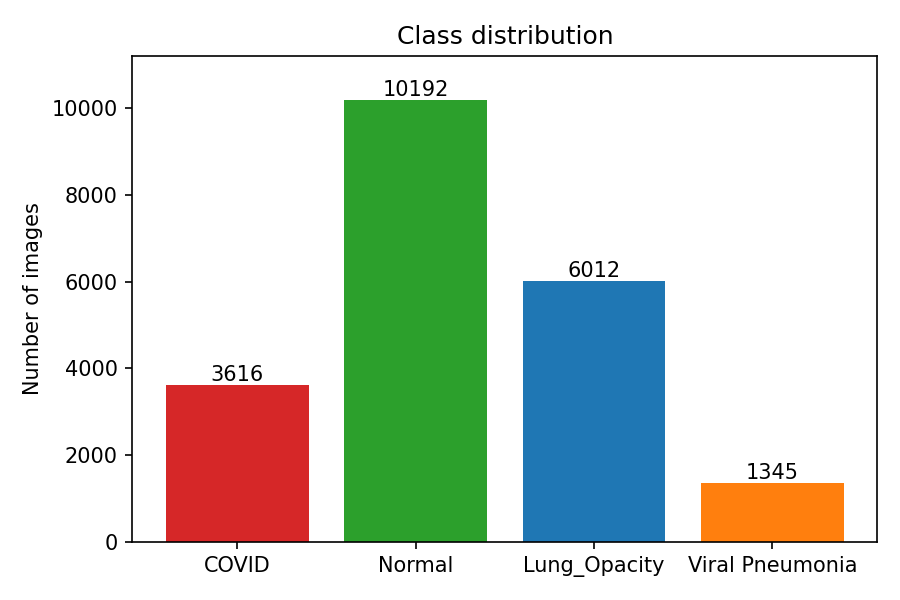
\includegraphics[width=0.75\textwidth]{figures/class_distribution.png}
    \caption{Distribution of chest X-ray images across the four diagnostic classes.}
    \label{fig:class_distribution}
\end{figure}

To determine whether the observed class frequencies differed significantly from
an equal class distribution, a chi-square goodness-of-fit test was performed.
The test indicated a highly significant deviation from uniformity
($\chi^2 = 8110.78$, $p < 0.001$). Furthermore, the effect size was large
(Cohen's $w = 0.619$), confirming the presence of substantial class imbalance.

The observed imbalance has important implications for model development and
evaluation. During dataset partitioning, stratified sampling should be employed
to preserve the original class proportions across the training, validation, and
test sets. Furthermore, overall classification accuracy alone may provide a
misleading assessment of model performance. Instead, evaluation should include
class-sensitive metrics such as per-class precision, recall, macro-averaged
F1-score, balanced accuracy, and the confusion matrix to ensure that
performance is assessed fairly across all diagnostic categories.

\section{Structural Integrity, Dimensions, and Image Encoding}

To verify the integrity of the dataset, all chest X-ray images and lung
segmentation masks were examined prior to model development. Every one of the
21,165 chest X-ray images had a corresponding segmentation mask with an
identical filename, indicating a complete one-to-one correspondence between
images and masks. Furthermore, no unmatched image--mask pairs or unreadable
PNG files were identified.

The average X-ray file size varied slightly across the four diagnostic classes.
The mean file sizes were 35.00 KB for COVID-19, 34.40 KB for Lung Opacity,
36.39 KB for Normal, and 39.36 KB for Viral Pneumonia. The relatively larger
mean file size observed for the Viral Pneumonia class is explained by the
presence of RGB images within this class, which are substantially larger than
their grayscale counterparts.

Table~\ref{tab:image_properties} summarizes the structural properties of the
dataset.

\begin{table}[H]
\centering
\caption{Structural properties of the chest X-ray images and segmentation masks.}
\label{tab:image_properties}
\begin{tabular}{lcc}
\toprule
\textbf{Property} & \textbf{X-rays} & \textbf{Masks} \\
\midrule
Number of files & 21,165 & 21,165 \\
Dimensions & $299 \times 299$ px & $256 \times 256$ px \\
L mode & 21,025 & 0 \\
RGB mode & 140 & 21,165 \\
\bottomrule
\end{tabular}
\end{table}

Although every image has a corresponding segmentation mask, the image and mask
dimensions differ. All chest X-ray images have a resolution of
$299 \times 299$ pixels, whereas all segmentation masks have a resolution of
$256 \times 256$ pixels. Consequently, any pixel-wise operation involving both
the X-ray image and its corresponding mask requires the mask to be resized or
otherwise aligned with the image dimensions.

\subsection{RGB Images in the Viral Pneumonia Class}

A detailed inspection of image encoding revealed that all 140 RGB images are
contained exclusively within the Viral Pneumonia class. These RGB images
represent 10.41\% of the Viral Pneumonia samples (140 of 1,345 images), while
every image in the remaining three diagnostic classes is stored as a
single-channel grayscale (L-mode) image. Consequently, image encoding is
associated with the diagnostic class in the raw dataset.

Table~\ref{tab:vp_encoding} summarizes the characteristics of the Viral
Pneumonia images according to image encoding.

\begin{table}[H]
\centering
\caption{Comparison of grayscale (L) and RGB images within the Viral Pneumonia class.}
\label{tab:vp_encoding}
\begin{tabular}{lrrrrr}
\toprule
\textbf{Mode} & \textbf{n} & \textbf{Mean (KB)} & \textbf{SD} &
\textbf{Median} & \textbf{Range (KB)} \\
\midrule
L & 1,205 & 37.45 & 2.54 & 37.47 & 26.37--47.27 \\
RGB & 140 & 55.82 & 5.86 & 56.28 & 39.83--71.42 \\
\bottomrule
\end{tabular}
\end{table}

Figure~\ref{fig:vp_filesize} compares the mean PNG file sizes of grayscale and
RGB images within the Viral Pneumonia class.

\begin{figure}[H]
    \centering
    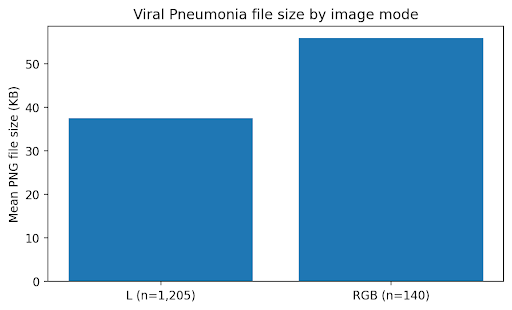
\includegraphics[width=0.75\textwidth]{figures/viral_pneumonia_file_size.png}
    \caption{Mean PNG file size of Viral Pneumonia images stratified by image encoding.}
    \label{fig:vp_filesize}
\end{figure}

As shown in Figure~\ref{fig:vp_filesize}, RGB images are substantially larger
than grayscale (L-mode) images within the same diagnostic category. This
finding indicates that the elevated average file size observed for the Viral
Pneumonia class is primarily attributable to differences in image encoding
rather than disease-related image characteristics.

Since image encoding represents a technical characteristic rather than a
clinically meaningful feature, all chest X-ray images should be converted to a
common grayscale representation during preprocessing. Standardizing the image
format eliminates a potential source of dataset bias and prevents the model
from exploiting encoding-related differences as shortcut features.

\section{Exact Duplicate Analysis}

To identify redundant images, perceptual hashing (pHash) was applied using a
Hamming-distance threshold of zero. This initial screening identified 287
candidate duplicate image pairs. A subsequent pixel-wise comparison confirmed
that 91 of these pairs were exact pixel duplicates, whereas the remaining 196
pairs shared an identical perceptual hash but differed at the pixel level. All
confirmed exact duplicates were found within the same diagnostic class, and no
duplicate images were shared across different class labels.

Duplicate images were subsequently grouped into connected duplicate sets, and a
single representative image was retained from each group. This process
identified a total of 59 redundant files, corresponding to only 0.28\% of the
entire dataset. The distribution of redundant files across diagnostic classes
is presented in Table~\ref{tab:duplicate_summary}.

\begin{table}[H]
\centering
\caption{Redundant exact duplicate files identified after grouping connected duplicate sets.}
\label{tab:duplicate_summary}
\begin{tabular}{lrr}
\toprule
\textbf{Class} & \textbf{Redundant Files} & \textbf{Percentage of Class} \\
\midrule
COVID-19 & 51 & 1.41\% \\
Lung Opacity & 0 & 0.00\% \\
Normal & 1 & 0.01\% \\
Viral Pneumonia & 7 & 0.52\% \\
\midrule
\textbf{Total} & \textbf{59} & \textbf{0.28\%} \\
\bottomrule
\end{tabular}
\end{table}

Figure~\ref{fig:duplicate_distribution} illustrates the number of confirmed
redundant images identified within each diagnostic class.

\begin{figure}[H]
    \centering
    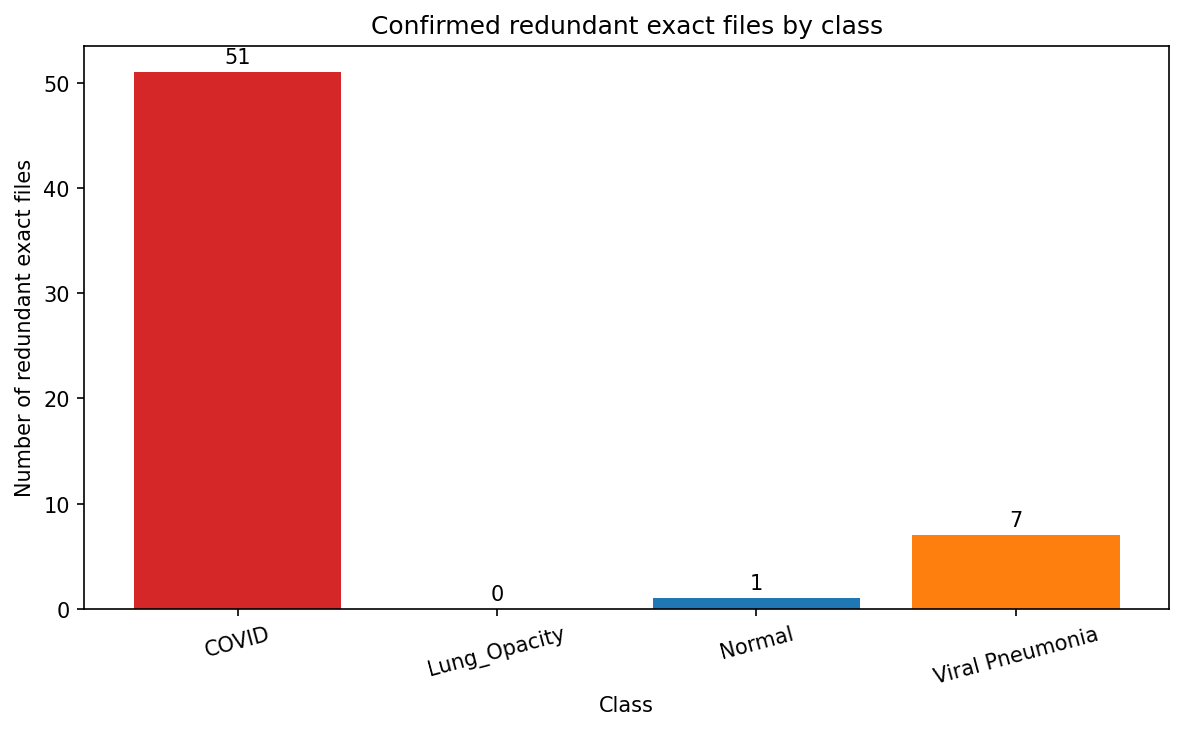
\includegraphics[width=0.75\textwidth]{figures/duplicate_distribution.png}
    \caption{Distribution of confirmed redundant exact duplicate files by diagnostic class after grouping duplicate sets.}
    \label{fig:duplicate_distribution}
\end{figure}

The identified duplicate images represent unnecessary redundancy within the
dataset and, if retained, could introduce data leakage by allowing identical
images to appear in both the training and evaluation sets. To prevent this
issue, the 59 redundant files were removed prior to performing the
training/validation/test split, while retaining one representative image from
each exact-duplicate group. This preprocessing step helps ensure an unbiased
evaluation of model performance and prevents overly optimistic performance
estimates resulting from duplicate observations.

\section{Whole-Image Brightness and Contrast}

To characterize global image intensity, two descriptive features were
calculated for each chest X-ray. \textit{Brightness} was defined as the mean
grayscale pixel intensity of the image, while \textit{contrast} was represented
by the standard deviation of grayscale pixel intensities within the image. To
ensure consistency, all chest X-ray images were converted to grayscale prior to
these calculations.

Table~\ref{tab:brightness_contrast} summarizes the descriptive statistics for
brightness and contrast across the four diagnostic classes. COVID-19 images
exhibited the highest mean brightness (139.52), whereas Normal images showed
the highest average global contrast (61.56). Lung Opacity and Viral Pneumonia
displayed similar central brightness values, although their contrast differed
slightly.

\begin{table}[H]
\centering
\caption{Descriptive statistics of whole-image brightness and contrast by diagnostic class.}
\label{tab:brightness_contrast}
\begin{tabular}{lcccccc}
\toprule
& \multicolumn{3}{c}{\textbf{Brightness}}
& \multicolumn{3}{c}{\textbf{Contrast}} \\
\cmidrule(lr){2-4}
\cmidrule(lr){5-7}
\textbf{Class}
& \textbf{Mean}
& \textbf{SD}
& \textbf{Median}
& \textbf{Mean}
& \textbf{SD}
& \textbf{Median} \\
\midrule
COVID-19        & 139.52 & 25.03 & 142.59 & 54.65 & 14.83 & 54.05 \\
Lung Opacity    & 126.02 & 23.57 & 120.82 & 57.40 & 9.81  & 56.97 \\
Normal          & 129.39 & 22.45 & 125.51 & 61.56 & 9.55  & 63.53 \\
Viral Pneumonia & 125.37 & 18.98 & 126.86 & 58.75 & 10.78 & 59.71 \\
\bottomrule
\end{tabular}
\end{table}

Figure~\ref{fig:brightness_boxplot} presents the distributions of brightness
and contrast for each diagnostic class. COVID-19 images tend to exhibit higher
overall brightness, whereas the Normal class has the highest global contrast.
The boxplots also reveal considerable within-class variability and numerous
statistical outliers, particularly for COVID-19. Since these measurements were
computed over the entire image, they may also be influenced by background
regions outside the lungs. Consequently, evaluating brightness and contrast
within the segmented lung regions may provide a more clinically meaningful
assessment.

\begin{figure}[H]
    \centering
    
\includegraphics[width=0.9\textwidth]{figures/brightness_contrast_boxplots.png}
    \caption{Whole-image brightness and contrast distributions by diagnostic class.}
    \label{fig:brightness_boxplot}
\end{figure}

Figure~\ref{fig:brightness_scatter} illustrates the relationship between
whole-image brightness and contrast. Although class-specific tendencies are
visible, substantial overlap exists among all four diagnostic classes.
COVID-19 images exhibit a broader spread in both brightness and contrast,
whereas Viral Pneumonia images are more tightly clustered. Normal images tend
toward higher contrast, consistent with the descriptive statistics shown in
Table~\ref{tab:brightness_contrast}. The considerable overlap indicates that
global intensity characteristics alone are unlikely to provide sufficient
discriminative information for reliable disease classification.

\begin{figure}[H]
    \centering
    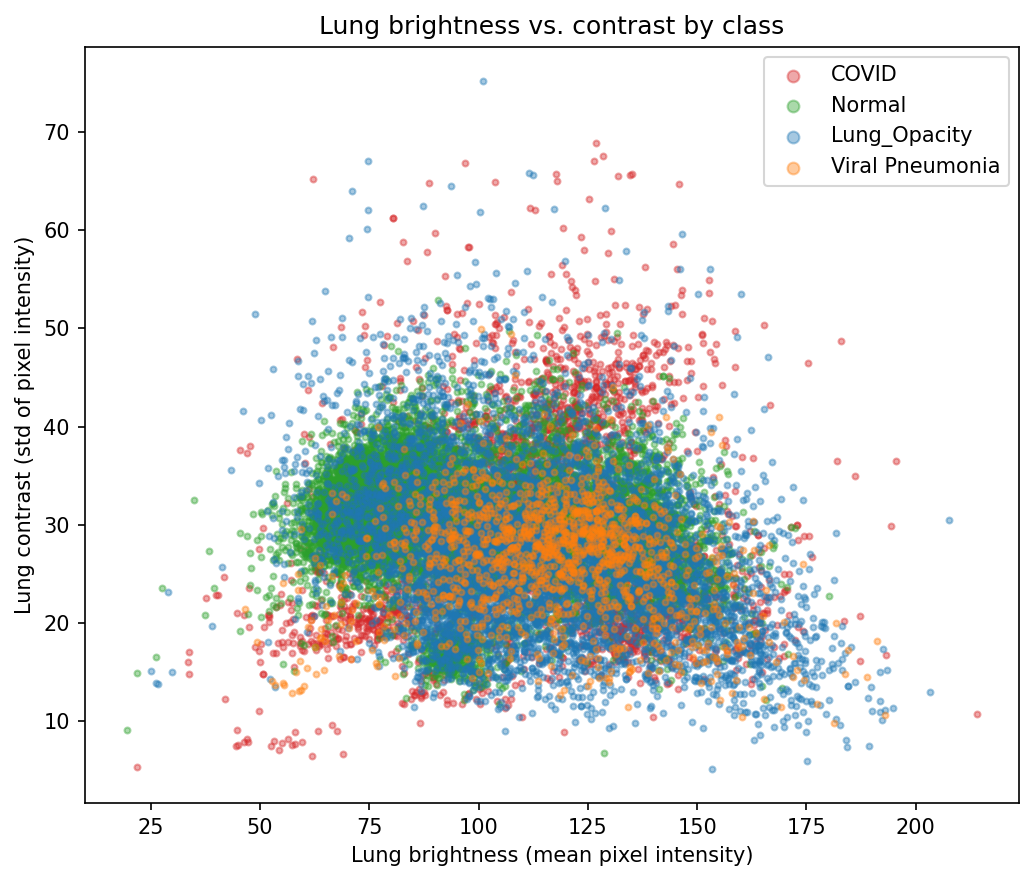
\includegraphics[width=0.8\textwidth]{figures/brightness_contrast_scatter.png}
    \caption{Relationship between whole-image brightness and contrast by diagnostic class.}
    \label{fig:brightness_scatter}
\end{figure}

The observed differences in global brightness and contrast are more likely to
reflect variations in image acquisition protocols, scanner characteristics, and
preprocessing procedures than disease-specific radiographic features.
Consequently, these global intensity characteristics may represent technical
confounding factors that a machine learning model could exploit as
\textit{shortcut features}. Applying intensity normalization during
preprocessing and evaluating its impact on model performance can help determine
whether the classifier relies on clinically meaningful radiographic patterns
rather than global intensity differences.

\subsection{Statistical Testing}

Non-parametric statistical analyses were performed to compare brightness and
contrast across the four diagnostic classes. A Kruskal--Wallis test indicated
significant differences in whole-image brightness
($H(3)=987.39$, $p<0.001$), with a small overall effect size
($\varepsilon^2=0.0465$). Significant differences were also observed for
whole-image contrast ($H(3)=1393.78$, $p<0.001$), with a modest effect size
($\varepsilon^2=0.0657$).

To quantify the magnitude of pairwise differences, Cohen's $d$ was computed for
each pair of diagnostic classes. The resulting effect sizes are summarized in
Table~\ref{tab:cohens_d}.

\begin{table}[H]
\centering
\caption{Pairwise Cohen's $d$ effect sizes for whole-image brightness and contrast.}
\label{tab:cohens_d}
\begin{tabular}{lcc}
\toprule
\textbf{Comparison} & \textbf{Brightness} & \textbf{Contrast} \\
\midrule
COVID-19 vs Lung Opacity            & 0.559  & -0.230 \\
COVID-19 vs Normal                  & 0.438  & -0.618 \\
COVID-19 vs Viral Pneumonia         & 0.601  & -0.296 \\
Lung Opacity vs Normal              & -0.147 & -0.431 \\
Lung Opacity vs Viral Pneumonia     & 0.029  & -0.135 \\
Normal vs Viral Pneumonia           & 0.182  & 0.290 \\
\bottomrule
\end{tabular}
\end{table}

Post hoc Dunn tests with Bonferroni correction revealed significant
brightness differences for every class pair except Lung Opacity versus Viral
Pneumonia. Although the comparison between Normal and Viral Pneumonia remained
statistically significant (adjusted $p = 0.0012$), the corresponding effect
size was small ($d = 0.182$). For whole-image contrast, all six pairwise
comparisons remained statistically significant following Bonferroni
adjustment. The largest standardized difference was observed between
COVID-19 and Normal ($d = -0.618$), indicating that COVID-19 images generally
exhibit lower global contrast than Normal images.

Overall, these findings demonstrate that brightness and contrast differ
systematically across diagnostic classes. However, the relatively small-to-
moderate effect sizes and substantial overlap among class distributions suggest
that global intensity characteristics alone are insufficient for robust disease
classification. Instead, they should primarily be regarded as potential
technical confounding variables that require careful preprocessing and
interpretation during model development.

\section{Summary of Current Evidence}

Table~\ref{tab:summary_evidence} summarizes the principal findings obtained
during the exploratory data analysis and their implications for the subsequent
preprocessing and model development stages.

\begin{table}[H]
\centering
\caption{Summary of key findings from the exploratory data analysis.}
\label{tab:summary_evidence}
\begin{tabular}{p{3cm} p{4.5cm} p{6cm}}
\toprule
\textbf{Domain} & \textbf{Main Result} & \textbf{Implication} \\
\midrule
Class balance &
$\chi^2(3)=8110.78$; Cohen's $w=0.619$ &
Substantial class imbalance, with the Normal class dominating the dataset and Viral Pneumonia being underrepresented. \\

Integrity &
0 unreadable files; 0 unmatched image--mask pairs &
Complete correspondence between chest X-ray images and segmentation masks. \\

Image encoding &
140 RGB X-rays, all belonging to the Viral Pneumonia class &
Class-specific technical artifact; all images should be standardized to grayscale before model training. \\

Exact duplicates &
59 redundant files, including 51 COVID-19 images &
Duplicate images should be removed prior to dataset partitioning to prevent data leakage. \\

Lung-mask coverage &
$H(3)=1493.59$; $\varepsilon^2=0.0704$ &
Modest but statistically significant differences in lung-mask coverage across diagnostic classes. \\

Whole-image brightness &
$H(3)=987.39$; $\varepsilon^2=0.0465$ &
Small but significant class-associated differences in global image brightness. \\

Whole-image contrast &
$H(3)=1393.78$; $\varepsilon^2=0.0657$ &
Modest but significant class-associated differences in global image contrast. \\
\bottomrule
\end{tabular}
\end{table}

Overall, the dataset is structurally complete and internally consistent.
However, several characteristics were identified that could influence machine
learning performance independently of clinically meaningful pathology. These
include substantial class imbalance, class-specific RGB image encoding,
concentrated exact duplication within the COVID-19 class, statistically
significant differences in lung-mask coverage, and systematic differences in
whole-image brightness and contrast across diagnostic categories.

Although these characteristics are not inherently problematic, they represent
potential technical confounding factors that could encourage a model to learn
dataset-specific shortcuts instead of disease-related radiographic features.
Consequently, the preprocessing pipeline has been designed to address these
issues through deduplication, image standardization, mask alignment, intensity
normalization, and stratified dataset partitioning. The effectiveness of these
preprocessing steps will be evaluated during model development to ensure that
the resulting classifiers learn clinically meaningful representations and
generalize reliably to previously unseen data.